% =======================================================================
% Checklist / TODO
% =======================================================================
% - [ ] Alterar o CDU (página 2)
% - [ ] Arrumar os dados da Folha de Registro do Documento (tg.tex)
% - [ ] Verificar se a data é a data da apresentação ou data da entrega do paper
% - [ ] Recolocar a Epígrafe
% - [ ] Tirei a dedicatório; Precisa para essa entrega?
% - [ ] Tirei o resumo (PT-BR); Precisa para essa entrega?

% - [ ] Colocar uma referência para o fork do scraper (https://github.com/cpbscholten/scraper)
% - [ ] Traduzir a figura de arquitetura
% - [ ] Colocar a referência do Firmadyne em todas as citações
% ======================================================================
% Começando com 9 páginas no template cru => ~5 páginas / por dia
% SEGUNDA (~15 páginas)
% - [x] Escrever capítulo de resultados
% - [ ] Escrever capítulo de arquitetura ou solução
% - [ ] Discutir as tabelas de estatísticas
% - [x] Colocar a imagem com o funil de sucesso
% TERÇA (~20 páginas)
% - [ ] Escrever capítulo de revisão bibliográfica (Aproveitar apresentação de CT-300)
% QUARTA (~25 páginas)
% - [ ] Escrever Considerações Finais e Próximos Passos
% QUINTA (~30 páginas)
% - [ ] Escrever Introdução (Destacar os objetivos <==> resultados)
% - [ ] Ajustar documento: abstract, títulos etc.


%%% exemplo de utilização da classe ita
%%%
%%%   por        fábio fagundes silveira   -  ffs [at] ita [dot] br
%%%              benedito c. o. maciel     -  bcmaciel [at] ita [dot] br
%%%              giovani volnei meinertz   -  giovani [at] ita [dot] br
%%%    	         hudson alberto bode       -  bode [at] ita [dot]br
%%%    	         p. i. braga de queiroz    -  pi [at] ita [dot] br
%%%    	         jorge a. b. gripp         -  gripp [at] ita [dot] br
%%%    	         juliano monte-mor         -  jamontemor [at] yahoo [dot] com [dot] br
%%%    	         tarcisio a. b. gripp      -  tarcisio.gripp [at] gmail [dot] com
%%%
%%%   versão para overleaf:
%%%   por           alejandro a. rios cruz - aarc.88@gmail.com
%%%                 saulo gómez            - sagomezs@unal.edu.co
%%%  importante: o texto contido neste exemplo nao significa absolutamente nada.  :-)
%%%              o intuito aqui eh demonstrar os comandos criados na classe e suas
%%%              respectivas utilizacoes.
%%%
%%%  tese.tex  2016-08-25
%%%  $headurl: http://www.apgita.org.br/apgita/teses-e-latex.php $
%%%
%%% italus
%%% instituto tecnológico de aeronáutica --- ita, sao jose dos campos, brasil
%%%                   http://groups.yahoo.com/group/italus/
%%% discussion list: italus {at} yahoogroups.com
%%%
%++++++++++++++++++++++++++++++++++++++++++++++++++++++++++++++++++++++++++++++
% para alterar o tipo de documento, preencher a linha abaixo \documentclass[?]{?}
%   \documentclass[tg]{ita}			= trabalho de graduacao
%   \documentclass[tgfem]{ita}	= para engenheiras
%   								msc     		= dissertacao de mestrado
%   								mscfem   		= para mestras
%   								dsc      		= tese de doutorado
%   								dscfem   		= para doutoras
%   								quali    		= exame de qualificacao
%   								qualifem 		= exame de qualificacao para doutoras
% para 'draft version'/'versao preliminar' com data no rodape, adicionar 'dv':
%   \documentclass[dsc, dv]{ita}
% para trabalhos em inglês, adicionar 'eng':
%   \documentclass[dsc, eng]{ita}
%		\documentclass[dsc, eng, dv]{ita}
%++++++++++++++++++++++++++++++++++++++++++++++++++++++++++++++++++++++++++++++
\documentclass[tg, eng, dv]{ita}    % ita.cls based on standard book.cls
% quando alterar a classe, por exemplo de [msc] para [msc, eng]) rode mais uma vez o botão build output caso haja erro
\usepackage{ae}
\usepackage{graphicx}
\usepackage{epsfig}
\usepackage{amsmath}
\usepackage{amssymb}
\usepackage{subfig}
\usepackage{multirow}
\usepackage{float}
\usepackage{amsthm}
\usepackage{url}         % formats url addresses properly
\usepackage{appendix}    % allows appendix section to be included
\usepackage{lscape}      % allows a page to be rendered in landscape mode
\usepackage{multicol}    % allows text in multi columns
\usepackage{cancel}      % needed to show canceled terms in equations
\usepackage{lettrine}
\usepackage{float}
\usepackage{placeins}
\usepackage[outputdir=latex.out]{minted}
\usepackage{prettyref}

\renewcommand\listingscaption{Código}

\newrefformat{anex}{Anexo~\ref{#1}}
\newrefformat{cap}{Capítulo~\ref{#1}}
\newrefformat{lst}{Código~\ref{#1}}
\newrefformat{tbl}{Tabela~\ref{#1}}

% Make ref autocomplete work.
\newcommand{\cref}[1]{\prettyref{#1}}

\usemintedstyle{friendly}

%HHHHHHHHHHHHHHHHHHHHHHHHHHHHHHHHHHHHHHHHHHHHHHHHHHHHHHHHHHHHHHHHHHHHHHHHHHHHHHHHHHHHHHHHHHHHHHHHHHHHHHHHHHHH
%\usepackage{subfigure}
%\usepackage{subfigmat}
%PACOTEFIGURAS_SE _ERRADO_ESXCLUIR_ACIMA
\usepackage{booktabs}
%PACOTETABELAS_SE _ERRADO_ESXCLUIR_ACIMA
%HHHHHHHHHHHHHHHHHHHHHHHHHHHHHHHHHHHHHHHHHHHHHHHHHHHHHHHHHHHHHHHHHHHHHHHHHHHHHHHHHHHHHHHHHHHHHHHHHHHHHHHHHHHH

%++++++++++++++++++++++++++++++++++++++++++++++++++++++++++++++++++++++++++++++
% Espaçamento padrão de todo o documento
%++++++++++++++++++++++++++++++++++++++++++++++++++++++++++++++++++++++++++++++
\onehalfspacing

%singlespacing Para um espaçamento simples
%onehalfspacing Para um espaçamento de 1,5
%doublespacing Para um espaçamento duplo

%++++++++++++++++++++++++++++++++++++++++++++++++++++++++++++++++++++++++++++++
% Identificacoes (se o trabalho for em inglês, insira os dados em inglês)
% Para entradas abreviadas de Professora (Profa.) em português escreva: Prof$^\textnormal{a}$.
%++++++++++++++++++++++++++++++++++++++++++++++++++++++++++++++++++++++++++++++
\course{Computer Engineering}

% Autor do trabalho: Nome Sobrenome
\authorgender{masc}
\author{Gianluigi}{Dal Toso}
\itaauthoraddress{H8A St., 111}{12228-460}{São José dos Campos--SP}

% Titulo da Tese/Dissertação
\title{Towards Router Firmware Analysis via Re-hosting}

% Orientador
\advisorgender{masc}
\advisor{Prof.~Dr.}{Lourenço Alves Pereira Júnior}{ITA}

% Coorientador
% \coadvisorgender{masc}
% \coadvisor{Prof.~Dr.}{Inaldo Capistrano Costa}{ITA}

%Coordenador do curso no caso de TG
\bosscoursegender{masc}
\bosscourse{Prof.~Dr.}{Johnny Marques}

% Palavras-Chaves informadas pela Biblioteca -> utilizada na CIP
%\kwcip{Cupim}

% Data da defesa (mês em maiúsculo, se trabalho em inglês, e minúsculo se trabalho em português)
\date{25}{JUNE}{2021}

% Número CDU - (somente para TG)
\cdu{XXX.XX}

% Glossario
\makeglossary
\frontmatter

\begin{document}
% Folha de Rosto e Capa para o caso do TG
\maketitle

% Dedicatoria: Nao esqueca essa secao  ... :-)
\begin{itadedication}
To my family, whose unconditional support was essential on my journey, and who always encouraged me and allowed me to pursue my dreams. 
\end{itadedication}

% Agradecimentos
% [DONE] TODO: Descomentar isso para o TG-2
\begin{itathanks}
% VER O MODELO DO DICKSIANO

% To Lourenço,

% \hspace{1em} explanation here...

% \hfill
% % ======================================================================

% To my family,

% \hspace{1em} explanation here...

% \hfill
% % ======================================================================

% To my girlfriend,

% \hspace{1em} explanation here...

% \hfill
% % ======================================================================

% To my friends and colleagues,

% \hspace{1em} explanation here...


\end{itathanks}

% Epígrafe
\thispagestyle{empty}
\ifhyperref\pdfbookmark[0]{\nameepigraphe}{epigrafe}\fi
\begin{flushright}
\begin{spacing}{1}
\mbox{}\vfill
{\sffamily\itshape
``Because the people who are crazy enough to think they \\
can change the world, are the ones who do.''\\}
--- \textsc{Steve Jobs}

\end{spacing}
\end{flushright}

% Resumo
\begin{abstract}
\noindent
% The widespread adoption of the home office weakens corporate networks, as it extends its perimeter to homes and ineffective security policies designed for different operating environments. In this context, wireless network routers serve as enablers of access to critical services. This is why studying embedded devices' software security is important to help vendors identify software flaws that lead to security vulnerabilities so they can fix them and enhance the security of their devices. This way, a large-scale cybersecurity attack leveraging insecure IoT devices can be avoided. However, identifying the software artifacts and possible vulnerabilities present on these devices is challenging. 

% One approach for inspecting the security of embedded firmware is to use system emulation to re-host the firmware execution to another machine from which security analysis can be performed. Nonetheless, firmware re-hosting is an open problem, motivating a lot of popular research on new techniques and approaches. This work aims to explore wireless router firmware security by enumerating its content to leverage information and statistics that enhance the performance of state-of-the-art re-hosting solutions for firmware analysis.

% To achieve this, we present our efforts in the analysis of $9176$ firmware images downloaded from $11$ vendors' sites and $3$ open-source firmware projects, yielding statistics of the most common operating systems and services present on these devices and automatically generating reports containing the most relevant information and important exposed files found on each firmware. Afterward, we present our results when trying to apply state-of-the-art solutions of re-hosting to some of our acquired firmware images.

A adoção em larga escala do trabalho remoto enfraquece as redes corporativas, visto que o perímetro desses redes é expandido para incluir domicílios e políticas ineficazes de segurança. Nesse contexto, roteadores de redes sem-fio servem como possibilitadores de acesso para serviços críticos. Por isso mesmo, estudar a segurança de \textit{software} de dispositivos embarcados é importante para auxiliar fabricantes a encontrar falhas de \textit{software} que causem vulnerabilidades de segurança, para estes consigam aplicar as devidas correções e aumentar a defesa de seus dispositivos.
Nesse sentido, pode-se evitar a ocorrencia de um ataque cibernético em larga-escala que se aproveite de dispositivos \textit{IoT} inseguros. No entanto, identificar os artefatos de \textit{software} e possíveis vulnerabilidades de segurança presente nesses dispositivos é desafiador.

%Nesse sentido, um ataque cibernético em larga-escala se aproveitando de dispositivos de \textit{IoT} inseguros pode ser evitado. 

Uma abordagem para a inspeção de segurança de \textit{firmwares} embarcados é utilizar a emulação ao nível de sistema para realizar a execução do \textit{firmware} em outra máquina a partir da qual análises de segurança possam ser realizadas. No entanto, o \textit{re-hosting} de \textit{firmwares} é um problema é aberto, e motiva diversas pesquisas recentes sobre novas técnicas e abordagens. Este trabalho visa explorar a segurança de \textit{firmwares} de roteadores sem-fio através da enumeração de seu conteúdo para o levantamento de informações e estatísticas que melhorem o desempenho das soluções estado-da-arte para a análise de segurança de \textit{firmwares} via \textit{re-hosting}.

Para isso, serão apresentados os esforços realizados para a análise de 9176 arquivos de \textit{firmware} obtidos dos \textit{websites} de 11 fabricantes e 3 projetos de \textit{firmware} de código-aberto, produzindo estatísticas dos serviços e sistemas operacionais mais presentes nesses dispositivos, além da geração automática de relatórios contento as informações mais relevantes e arquivos expostos encontrados em cada \textit{firmware}. Posteriormente, serão também apresentados os resultados obtidos a partir da aplicação das ferramentas estado-da-arte para a execução de \textit{re-hosting}, nos arquivos de \textit{firmware} obtidos.
\end{abstract}

% Abstract
\begin{englishabstract}
\noindent
TODO

% OLD ABSTRACT, NEED TO DO A NEW ONE AFTER THE WORK IS DONE

% Studying embedded devices software security is important to help vendors identify software flaws that lead to security vulnerabilities so they can fix them and enhance their devices security. This way, a cybersecurity attack leveraging insecure IoT devices can be avoided. In this preliminary work we describe a way to automate security analysis on wireless routers firmware. Our proposal is to automatically acquire firmware images from vendor websites, extract kernel and filesystem from the acquired images and then re-host the firmware inside an emulator to use known techniques of vulnerability discovery.


\end{englishabstract}

% Lista de figuras
\listoffigures %opcional

% Lista de tabelas
\listoftables %opcional

% Lista de abreviaturas
\listofabbreviations
\begin{longtable}{ll}
  IoT & \textit{Internet of Things} \\
  SOHO & \textit{Small Office/Home Office} \\
  ROM & \textit{Read-Only Memory} \\
  EPROM & \textit{Erasable Programmable Read-Only Memory} \\
  EEPROM & \textit{Electrically Erasable Programmable Read-Only Memo} \\
  SD & \textit{Secure Digital} \\
  BIOS & \textit{Basic Input/Output System} \\
  HDD & \textit{Hard Disk Drive} \\
  CPU & \textit{Central Processing Unit} \\
  KVM & \textit{Kernel-based Virtual Machine} \\
  OS & \textit{Operating System} \\
  CRS & \textit{Cyber Reasoning Systems} \\
  API & \textit{Application Programming Interface} \\
  PNG & \textit{Portable Network Graphics} \\
  PDF & \textit{Portable Document Format} \\
  SoC & \textit{System on a Chip} \\
\end{longtable}

 %opcional

% Lista de simbolos
%\listofsymbol
%\begin{longtable}{ll}
\end{longtable}

 %opcional

% Sumario
\tableofcontents


\mainmatter
% Os capitulos comecam aqui

\chapter{Introduction}
In the last decades, the ability to work in a person's home has been an increasing desire in society, and following the fast advances in technology, companies were already experimenting with remote models of work. Amidst the COVID-19 pandemic, many cities imposed mobility restrictions in order to restrain virus spreading.  Henceforth, companies have adopted remote work, and there is a tendency to increase this model considerably in a pos-covid world.

Working from home expands the companies' network perimeter, exposing digital assets to new threats and vulnerabilities. Consequently, it causes an increase in a company's attack surface as small and home office types of equipment are potentially more vulnerable. Home wireless routers, for instance, are the worker's first access to the internet and maybe running firmware with security breaches that could leverage to provoke a cybersecurity incident.

One approach is to detect vulnerabilities in firmware products before the attackers and report them back to the vendor to prevent this kind of attack. Thereby, the manufactures can patch the system to fix the identified security breaches. This paper aims to discuss a way to automate the security analysis and vulnerability detection in wireless router firmware via re-hosting the original firmware in an emulator before executing vulnerability analysis and discovery techniques.

\chapter{Background}
\section{Firmware}

Firmware is a class of computer software that is built for a specific embedded hardware with the goal to provide basic functionalities and act as an operational system. Firmware can be very different from each other and may vary greatly between vendors. Usually firmware is part of the equipment and is held in the device's non-volatile memory, such as ROM, EPROM, EEPROM and flash memory. In this research work, we focus our attention in wireless router firmware and most specifically in those who are based on the Linux operating system.

\section{Re-Hosting}

Re-hosting specifies that a binary that would run on a specific hardware is instead run on a host system using system emulation and is therefore ``re-hosted'' \cite{firmware-challenges}. Firmware re-hosting in this context relates to executing the firmware, that was originally designed to run on the original hardware, on a desktop computer (i.e. not in the physical hardware it was designed to). Re-hosting challenges involve executing binaries that were designed to run on a specific processor architecture on another. This is usually done using an emulator software.

One very popular open source tool for architecture emulation is the QEMU framework, that does dynamic binary translation: guest CPU instructions are converted to the host CPU instructions, converting them to work with the change in CPU architecture. QEMU is a complex tool that implements a lot of optimizations to this translation process. It also leverages Linux kernel features from the host (if available) to enhance emulation speed.

\section{Software Vulnerability}

Although there are many ways to describe a software vulnerability, one that is close to the software engineering field is that a software vulnerability is an instance of a mistake in the specification, development or configuration of software such that its execution can violate the explicit or implicit security policies \cite{vuln-discovery}. By this definition, one mistake can incur in different vulnerabilities inside a software product.

Companies have put increasingly effort on the adoption of secure software development techniques in early stages of product implementation in order to avoid making mistakes that can lead to vulnerabilities. Even so, software development is a really extensive task and even experienced developers can sometimes make mistakes.

Software vulnerabilities may be exploited by malicious actors to gain access to damage a product or to gain access to sensitive information. Therefore, it is important for companies and security researchers to have effective ways to find vulnerabilities within their products, so that they can update the product to patch these vulnerabilities and provide more security to their business and to their customers. Efficiency in this process is also highly desirable as the latter vulnerabilities are discovered, it becomes more and more expensive to remediate them \cite{soft-eng-economics}.

\subsection{Vulnerability Discovery}
\label{subsec:vuln-disc}

Given the importance of the vulnerability discovery process, some techniques were developed to assist human specialists in this process and these techniques are moving towards becoming more and more automated, such as in the future we may have complete Cyber Reasoning Systems (CRS) working in this process of vulnerability disclosure \cite{crs}.

Nowadays, human specialists are still the main source of vulnerability discovery and the main techniques used in this process are: static analysis, dynamic analysis, symbolic execution and fuzzing. In the following subsections, we will briefly explain how each of these techniques work, and in Table \ref{tab:disc-techniques} we compare these techniques \cite{fuzzing}.

\begin{table}[h]
    \centering
    \caption{Comparison between vulnerability discovery techniques}
        \begin{tabular}{|c|c|c|c|}
        \hline
        \textbf{Technique}   & \textbf{Initial Complexity} & \textbf{Accuracy} & \textbf{Scalability} \\ \hline
        Static Analysis    & Easy      & Low   & Good         \\ \hline
        Dynamic Analysis   & Hard      & High  & Uncertain    \\ \hline
        Symbolic Execution & Hard      & High  & Bad          \\ \hline
        Fuzzing            & Easy      & High  & Good         \\ \hline
        \end{tabular}%
    \label{tab:disc-techniques}
\end{table}

\subsubsection{Static Analysis}

Static analysis consists in searching for vulnerabilities in a software without really executing its code. Static analysis is performed by searching the source code (it can be the object code too, but is a lot harder) for known syntax that may lead to bugs. Static analysis can be automated and tools can be quickly used to search inside a codebase for semantics that appear to be vulnerable. The downside of static analysis is that its simplistic approach is prone to result in a lot of false-positives, and it requires some specialist to read the automated reports to filter the results.

As this analysis is easily automated and quick to execute, it is best used during the development process, and may be even incorporated to the software production pipeline.

\subsubsection{Dynamic Analysis}

In contrast to static analysis in which the software is not executed, dynamic analysis is the process of searching for vulnerabilities in a software during its execution. Software state and execution flow can be monitored during software execution, and a human specialist with strong technical skills in analysis can use this monitored execution environment to find bugs precisely. That being said, this technique is extremely accurate, but also very dependent on the intervention of a human with strong technical skills, restraining the automation of this kind of analysis.

\subsubsection{Symbolic Execution}

Symbolic execution can be considered a specific form of automated dynamic analysis in which the program is executed in a controlled and instrumented environment and each input read by the program is treated as a symbol. When the assembly code reaches a branch instruction that depends on the value of this symbol, then the program takes note of each value constraints for each symbol. This way, knowing every symbol and constraint equation, a symbolic solver could be used to map values for the symbols in such way that every code flow is reached.

This method has been proven to be extremely accurate in small, simple programs. However, when the code grows, the symbolic execution faces the \textit{path explosion} problem. The number of possible paths becomes so big that it becomes impossible for the solvers we have available to calculate every execution flow.

\subsubsection{Fuzzing}

Fuzzing can also be considered a specific form of an automated dynamic analysis. This technique consists of generating a massive amount of normal and abnormal inputs and feeding the target program with these generated inputs. Execution state is then monitored to identify if any of the inputs corrupted the execution flow. Fuzzing technique is easy to be deployed, with high accuracy as it is done in the real execution, and also easy to be scaled. However, fuzzing still has issues with low efficiency and code coverage, but as it is also a relatively new technique, a lot of research is being developed upon enhancing this technique, that has already become the state-of-art vulnerability discovery technique currently \cite{fuzzing}.


\subsection{Challenges in Vulnerability Discovery for IoT}

Regarding the vulnerability discovery methods presented in section \ref{subsec:vuln-disc}, these methods were developed to find vulnerabilities in general purpose computers such as home computers or servers. When trying to discover vulnerabilities in software developed for embedded hardware, researchers may face additional challenges.

The first challenge may be the acquisition of the target software. Many firmware images were only developed to work within their original hardware, and the only way to have a copy of the software may be opening the hardware and extracting the original system from one of its memories.

Another challenge is the dependency of the hardware. Firmware images are usually tied to the original hardware they were designed to operate with. To apply vulnerability discovery techniques in firmware files, we have to re-host the firmware so that it can be run inside an emulator and there we can apply the vulnerability discovery techniques. Usually, re-hosting is a process with a lot of challenges by its own.

An additional challenge presented by firmware images that don't use a general purpose operating system (such as Linux, FreeRTOS, VxWorks) or firmwares that are really lean is that the vulnerability discovery methods aforementioned rely on monitoring operating system calls that indicate memory corruption. If the firmware don't implement security mechanisms that indicate memory corruption, it becomes a lot harder to automatically detect that the firmware execution reached an abnormal state (caused by the exploitation of an existent vulnerability) \cite{wycinwyc}.

\chapter{Related Work}
Regarding how to overcome re-hosting difficulties caused by the need of peripherals of the original hardware that are not present in the emulated device, researchers have developed different approaches. The work of \cite{firmware-challenges} surveys the most prominent techniques used in firmware re-hosting to bypass real hardware dependency. The four most common approaches are: Partial Emulation, Fuzzing, Learning and Abstraction Replacement.

\section{Partial Emulation}

Partial emulation, also known as ``hardware in the loop'' consists of emulating most part of firmware execution, but redirecting to the real device hardware calls when the firmware asks for a peripheral that can't be emulated. This approach requires having a real device available, and for this reason it does not scale. Execution fidelity in other hand is pretty close to the real hardware execution. The work of \cite{surrogates} enhances hardware redirecting by building a hardware bridge using an FPGA board to connect the PCI bus on the emulating host with the PCI bus on the real embedded device, an approach they called {\tt SURROGATES}.

The work of \cite{avatar2} greatly explores vulnerability discovery in embedded devices using the hardware in the loop technique. They use a symbolic engine build upon QEMU called {\tt S2E} to search for vulnerabilities in IoT devices through re-hosting and redirecting peripherals calls to the real hardware. They implement a tool called {\tt Avatar²} as a reverse engineering framework based on hardware in the loop approach.

\section{Fuzzing}

Fuzzing as a re-hosting approach to hardware dependence (not to be confused with fuzzing as a vulnerability discovery technique) is based on the fact that hardware calls to peripherals don't really need the peripheral to be successful. The real peripheral ``answer'' to the hardware call is just a binary value. Knowing the range of values that provide an accepted answer to the hardware call, selecting any random value withing this range will be enough to keep executing the emulated system.

One way to effectively implement this kind of hardware bypass is proposed in the work of \cite{p2im} in which the authors present an approach to model the interface between the processor and the peripheral. The method suggested is called {\tt P2IM} - Processor-Peripheral Interface Modeling, and it requires a human specialist to model the interface between the CPU and a specific peripheral in order to determine the specific range of values to each hardware call.

As this approach required human intervention (to model the interface) it is also not a scalable solution.

\section{Learning}

Learning is a similar approach to fuzzing for re-hosting, as it relies on the fact that to bypass hardware dependence it is only needed to return expected values to hardware calls. However, the learning approach, as used in \cite{pretender} first monitor real hardware execution and registers each hardware-peripheral interaction. Then it uses a Machine Learning algorithm to build a model of the interface (in contrast to using a human specialist as in the fuzzing approach). Learning technique produces a better interface to simulate peripheral interaction, but it also depends on having the real hardware first to build the working model of the interface, and that also impede its scalability.

\section{Abstraction Replacement}

Abstraction Replacement takes a different approach and instead of trying to produce answers to hardware calls that are similar to the answers a real hardware would produce, this method tries to completely remove from the original firmware the hardware call, replacing it with another abstraction that does not require the real hardware.

In the work of \cite{halucinator}, they develop the method called {\tt Halucinator}, whose idea is to search for Hardware Abstraction Layer (HAL) libraries inside the firmware and replace those libraries with custom libraries implemented by the researchers that do not require peripherals to work. This method still require human intervention for each firmware and thus, does not scale.

In the other hand, the work of \cite{firmadyne} implements a tool called {\tt Firmadyne}, whose approach to re-hosting consists of replacing the original kernel found on the firmware image with a custom implemented and instrumented kernel worked by their team (the same kernel is used to all firmware images emulated, regardless their original kernel version). They can then emulate firmware at scale, with the counterpart that the kernel replacement sacrifices emulation fidelity.

%\subsection{Firmadyne}

\chapter{Methodology}
In this chapter, we will present the architecture our research proposes in order to evaluate the large-scale re-hosting of router firmware images and the innovative aspects of the approach intended in this project.

\section{Complete Architecture}
This paper represents only part of a solution idealized for a bigger research project, to be conducted throughout the years by a team of researchers. Figure \ref{fig:architecture} illustrates the overview of the architecture for the complete project, whereas in this paper we will only focus on the re-hosting part of the proposed architecture.

\begin{figure}[h]
    \centering
    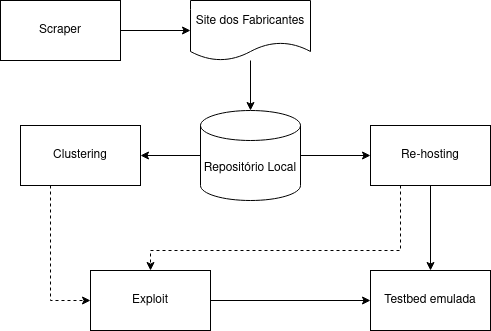
\includegraphics[width=0.65\textwidth]{figs/RehostingDiagram.png}
    \caption{Architecture proposed for a complete solution in firmware vulnerability analysis.}
    \label{fig:architecture}
\end{figure}

The complete architecture includes a scraper module consisting of a web crawler responsible for entering router vendors websites and downloading for a local repository the biggest amount of firmware images available as possible. Firmware images are going to be a requirement for the re-hosting experiments to be conducted. In this stage, the scraper module is going to only serve the purpose of providing a minimum amount of firmware images to allow the research in the re-hosting process. Therefore, our approach will be to use Firmadyne's \cite{firmadyne} implemented scraper for now. In the future, if needed, our team is willing to update Firmadyne's \cite{firmadyne} scraper and also add more vendors to the list.

From the local repository, two different modules will perform actions using the acquired firmware. The re-hosting module will be responsible for extracting firmware images (and collecting information about the firmware in the process) and preparing the firmware image to be emulated. As this module will be the focus of this research, section \ref{sec:re-hosting} will explain this process in detail. The other module to perform actions in firmware images contained in the local repository is the clustering module. This consists on searching for similarities and patterns amongst different firmware images. The results obtained by the clustering modules can be used in further steps to improve the vulnerability analysis and discovery process.

The final module of the architecture is the exploitation module. In this stage, vulnerability analysis (using frameworks to detect known software vulnerabilities) and vulnerability discovery (such as fuzzing techniques) will be applied on the emulated firmware to analyze its security performance.

\section{Firmware Extraction}
\label{sec:extraction}

For the firmware extraction process, our research is going to focus on enhancing the original script provided with Firmadyne \cite{firmadyne} for firmware extraction developed in Python and making extensive use of {\tt binwalk}'s API. This original script uses {\tt binwalk} to recursively extract the firmware image setting a limit for depth and breadth in order to limit this process as it is very slow. To speed up the extraction, the {\tt /tmp} directory of the host system (which is used to temporarily store files during the firmware extraction process) is going to be mounted on the {\tt tmpfs} provided by the Linux kernel and that allow us to mount a directory in the RAM instead of mounting it on the disk.

Some firmware images can't be automatically extracted using this method. After executing the script in all firmware images, we will then check which were not successfully extracted in the automated process. Some of these will be manually extracted in order to identify if and how the extraction process could be modified to be able to also extract this image. After modifying the extraction script, this entire process will be repeated until our team is satisfied with the amount of extracted firmware images.

\section{Re-hosting Process}
\label{sec:re-hosting}

During the re-hosting phase, our objective is to be able to run software intended to run in the original firmware without really having the original hardware in which it was designed to run. Firmadyne's \cite{firmadyne} approach to firmware re-hosting is to extract from the original firmware image its original root filesystem and kernel. It then completely ignores the original kernel, and replace it with a custom instrumented kernel designed by the researchers (they developed one instrumented kernel for {\tt ARM} architecture and one for {\tt MIPS} architecture). Finally, the emulation process is done by the {\tt QEMU} tool, that uses binary translation to allow execution of binaries from different architectures. The emulated firmware is emulated with {\tt QEMU} using the instrumented kernel together with the extracted filesystem from the original firmware.

Our approach to firmware re-hosting will be similar to Firmadyne's \cite{firmadyne} approach, with differences in regard to the kernel replacement part. Instead of just building one heavily instrumented kernel and replacing all firmware images with that same instrumented kernel, we propose building specific kernel versions on demand according to the original kernel used by the firmware image being emulated. With that, our hope is that using a kernel more similar with the original one could reduce incompatibility with network drivers and modules and therefore increase the number of emulated firmware with a working network interface, allowing us to extend the vulnerability analysis and discovery process to a bigger amount of router firmware images than the one covered by the original Firmadyne's \cite{firmadyne} implementation.

This process of automated kernel cross-compilation, however, faces a lot of issues. The first one is how to define a valid kernel compile configuration that results in a kernel that has the features expected in a router firmware. Kernel compile configuration is a configuration file ({\tt .config}) where the user can configure a large list of parameters regarding the kernel that will be compiled.

These configuration files can be filled up by the user manually or via answering questions interactively in the command line interface, or it can also be extracted from an already existing compiled kernel in execution. Defining how to produce an adequate {\tt .config} file is already an open problem in our research. Other idea is to extract kernel compilation default configuration from OpenWrt Linux systems. The OpenWrt is a Linux developed to be used as an open-firmware for wireless routers. That being said, it is possible that OpenWrt images have kernel configurations that are compatible with most networking features expected from a wireless router. In this way, in this research, we plan to investigate the better way to produce a valid compilation configuration file in order to allow kernel compiling.

After choosing a valid kernel compilation configuration file, the kernel has to be cross-compiled in the host machine, so that it is compiled for the architecture expected in the original firmware image. Kernel cross-compilation is also a very difficult task, as the compilation process is heavily dependent on its toolchain (compiler, utilities and libraries versions). This means that in order to automatically compile multiple different kernel versions, there has to be a way to automatically switch between a set of known working toolchains for each kernel version.

Finally, after compiling a kernel version that matches the original kernel, the firmware image is then ready to be emulated using the {\tt QEMU}. Firmware will be emulated using the newly compiled kernel with the original filesystem extracted from the firmware sample. After that, following the work of \cite{firmadyne}, we will evaluate if these emulated firmware images can infer and configure the network successfully. If that is the case, then vulnerability analysis and discovery techniques will be applied (using common tools for this purpose). The results obtained will be used to evaluate overall firmware security and the mapped vulnerable products (if that happens) will be reported back to the vendor.

\chapter{Results}
In this chapter, we will discuss the obtained results in the process of firmware acquisition and firmware extraction, previous steps before the actual firmware re-hosting.

\section{Firmware acquisition}

For the firmware acquisition, we used a fork of the Firmadyne's \cite{firmadyne} original scraper \cite{github:scraper}. This modified scraper version has fixed some compatibility issues the original scraper has with Python 3 and also updates the spiders to match more updated version of vendor websites. Without modifying any of the spiders provided by the scraper, we selected five vendors and executed the scraper to automatically find and download firmware from these vendors websites. In total, 5265 firmware images were downloaded throughout this process. Table \ref{tab:scraper} show the amount of firmware images and its combined file size for each vendor.

\begin{table}[h]
\centering
\caption{Downloaded firmware images per vendor}
\begin{tabular}{|c|c|c|}
\hline
\textbf{Vendor} & \textbf{Firmware Images} & \textbf{Combined File Size} \\ \hline
Netgear         & 3122                     & 93 GB                       \\ \hline
TP-Link         & 1320                     & 10 GB                       \\ \hline
D-Link          & 430                      & 6.7 GB                      \\ \hline
Ubiquiti        & 226                      & 20 GB                       \\ \hline
Tenda           & 167                      & 1 GB                        \\ \hline
\end{tabular}
\label{tab:scraper}
\end{table}

As the goal of this work is towards the process of re-hosting, this amount of firmware images is already enough for initial experiments with automated re-hosting. In further work, more vendors pages can be extracted, and we can update scraper's spiders if we judge there is need for a larger volume of firmware images.

\section{Firmware extraction}

Firmware extraction was heavily based on the usage of the {\tt binwalk} tool, whose usage was wrapped inside a script provided by Firmadyne \cite{firmadyne}. This script, when executed with a firmware image as a parameter, recursively tries to extract files using {\tt binwalk} for this purpose. It defines a breadth and depth limit to this recursion strategy. During the extraction process, the script then tries to identify if any of the extracted directories has a Linux root directory structure (i.e. has {\tt /bin}, {\tt /etc}, {\tt /usr} directories and so on). If that is the case, then this filesystem structure is compressed and stored in a separate location (also defined as a parameter to the script). 51.17\% of the total amount of firmwares (2694 images) were successfully extracted by Firmadyne's \cite{firmadyne} extraction script. Of these extracted images, 48.52\% (1307 images) had the filesystem extracted and of these, 83.55\% (1092 images) had the architecture identified. Architecture identification is done by reading files in filesystem directories that should contain binary files (e.g. {\tt /bin} or {\tt /sbin}) and reading the header of these files.

Kernel detection is done by reading each entry identified by {\tt binwalk} in the extraction process and detecting known kernel types. These are also extracted and stored in a separate location. When using the script, the user has the option to disable kernel extraction, as this greatly improves execution speed since {\tt binwalk} spends a lot of effort in the extraction process. If kernel extraction is not disabled by user, then the script also tries to identify kernel version and store this information in Firmadyne's \cite{firmadyne} database if found.

As not all kernels are identified by the described process above, we also developed an additional script that uses regular expressions to search the extracted filesystem of each firmware image with a non identified kernel during extraction and for directories that could reveal kernel version (e.g. {\tt /lib/modules/2.6.31} is an indicative that this image contains a 2.6.31 Linux kernel). This search is extremely fast compared to the filesystem extraction process and increased the number of kernel versions detected. Initially, with the Firmadyne's \cite{firmadyne} original extraction script, 983 kernels were identified amongst the 2694 (36.49\%) of the total amount of firmware images. After running the described heuristics to determine kernel version from filesystem, the number of identified kernels increased to 1169 (18.92\% greater).

\begin{figure}[h]
    \centering
    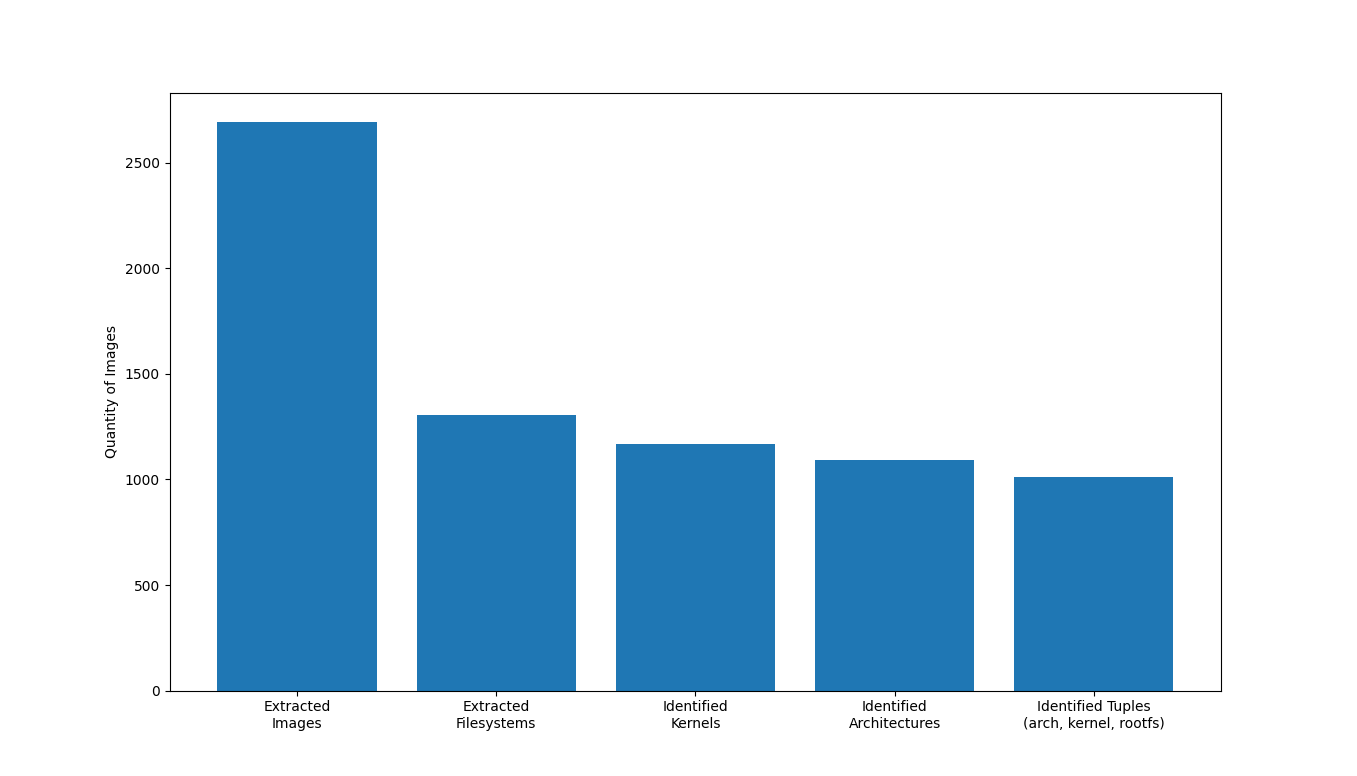
\includegraphics[width=0.90\textwidth]{figs/Funnel.png}
    \caption{Success funnel for firmware image extraction.}
    \label{fig:stats-funnel}
\end{figure}

It was also identified two issues in the extraction process. Some kernel image media types (formerly known as MIME types) were incorrectly identified as a type that was on the extraction script blacklist. This could be easily corrected excluding the identified type from the blacklist. The second issue is related to the recursive extraction process. The limits in breadth and depth exploration allow the {\tt binwalk} tool to have usable performance, but in some cases these limits were in fact responsible for the firmware extraction to be unsuccessful. Therefore, we believe using an heuristic to select files with the most potential to hold firmware kernel or filesystem to be extracted next. This way we can still have breadth and depth limits to maintain the extraction process feasible but it would also focus the extraction in files that are more prominent. This approach of using an heuristics although idealized was not yet implemented in our work.

Another enhancement we developed to the extraction process was the ability to extract addition kernel information. During kernel extraction, the kernel binary file is scanned for ASCII strings and from the result of this search we then extract kernel banner (a string containing kernel version, compiler version used during kernel compilation, compilation date and email of the developer who compiled the kernel) or identify for instance if the system being extracted refers to an OpenWrt Linux. These additional pieces of information are also stored in Firmadyne's \cite{firmadyne} database, that had its schema altered to contain a new column to store the extra information for a given firmware image.

% Falar das estatísticas; Colocar tabela com as estatísticas

\subsection{Statistics}

Regarding firmware extraction and feature identification, we collected some statistics that may help the following steps of this work in kernel compilation and firmware re-hosting. Table \ref{tab:arch-stats} shows the amount of firmwares detected for each architecture identified. Tables \ref{tab:kernel-stats} and \ref{tab:kernel-family-stats} shows the five most common kernel versions and kernel families respectively.

\begin{table}[h]
\centering
\caption{Number of images identified for each found architecture}
\begin{tabular}{|c|c|}
\hline
\textbf{Architecture} & \textbf{Quantity of Images} \\ \hline
{\tt mipseb}                & 485                         \\ \hline
{\tt armel}                 & 336                         \\ \hline
{\tt mipsel}                & 249                         \\ \hline
{\tt mips64eb}              & 11                          \\ \hline
{\tt ppceb}                 & 10                          \\ \hline
{\tt intel64el}             & 1                           \\ \hline
\end{tabular}
\label{tab:arch-stats}
\end{table}

\begin{table}[h]
\centering
\caption{Five most common kernel versions found in extracted firmwares}
\begin{tabular}{|c|c|}
\hline
\textbf{Kernel Version} & \textbf{Quantity of Images} \\ \hline
2.6.31                  & 167               \\ \hline
2.6.36                  & 122               \\ \hline
3.3.8                   & 46                \\ \hline
3.14.77                 & 44                \\ \hline
2.6.22                  & 44                \\ \hline
\end{tabular}
\label{tab:kernel-stats}
\end{table}

\begin{table}[h]
\centering
\caption{Five most common kernel families found in extracted firmwares}
\begin{tabular}{|c|c|}
\hline
\textbf{Kernel Family} & \textbf{Quantity of Images} \\ \hline
2.6                    & 484               \\ \hline
3.14                   & 63                \\ \hline
3.3                    & 46                \\ \hline
3.10                   & 38                \\ \hline
3.4                    & 33                \\ \hline
\end{tabular}
\label{tab:kernel-family-stats}
\end{table}

% Dissertar sobre as tabelas

\section{Kernel Cross-compilation \& Toolchain Building}

As shown by Table \ref{tab:kernel-family-stats}, kernel family 2.6 was the most commonly found amongst successfully extracted kernels. Therefore, we investigated the difficulties of cross-compiling a 2.6 Linux kernel. At first, we tried to cross-compile the kernel in a raw modern operating system. We chose Debian 10 (running with Linux kernel version 4.19) as the starting point for this experiment. In this environment, with {\tt gcc} version 8.3.0 as the compiler and using {\tt libc} version 2.28.10 it was not possible to compile the target kernel.

Then we downloaded an old version of the Debian operating system, with a release date similar to the 2.6 Linux kernel. Debian 3.1r8 (kernel 2.4.27) was used for this experiment. Using this old operating system, with {\tt gcc} version 3.3.5 as the compiler and using {\tt libc} version 2.3.2, we had success in compiling the target kernel.

This highlights the impact the toolchain (compiler, binary utilities and library versions) has on kernel compiling process and therefore to achieve a way to automate kernel compiling, we also need a way to automate toolchain building. In this context, we adopted the {\tt crosstool-ng} tool. With this program, the user can define, between some pre-configured settings, specific versions for each tool inside the toolchain, and the program then tried to compile the desired toolchain.

Using {\tt crosstool-ng} we were then able to successfully compile a 2.6 Linux kernel inside a Debian 10 (modern operating system). However, when trying to cross-compile the target kernel for the {\tt MIPS} architecture (cross-compiling), we still faced issues that did not allow the kernel to compile successfully and further investigation is needed in order to build a working toolchain for this scenario.

\chapter{Future Work}
The work described in this document is part of an ongoing research project and its purpose is mostly to describe the approach we intend to use during the research. That being said, the main research and implementation is yet to happen next semester. The following section presents the next planned steps and schedule for this research work:

\section{Activities Schedule}

\begin{enumerate}
    \item Finish work environment setup and firmware acquisition process.
    \begin{itemize}
        \item Expect to finish until the end of \textbf{June, 2021};
    \end{itemize}

    \item Enhance firmware extraction process.
    \begin{itemize}
        \item Expect to finish until mid \textbf{July, 2021};
    \end{itemize}
    
    \item Setting up a toolchain building for kernel cross-compilation.
    \begin{itemize}
        \item Expect to finish until the end of \textbf{July, 2021};
    \end{itemize}
    
    \item Re-host firmware images using the compiled kernels and fix incompatibilities
    \begin{itemize}
        \item Expect to finish until mid \textbf{September, 2021};
    \end{itemize}
    
    \item Enhance the re-hosting process and evaluate the emulated firmware performance regarding its network capabilities \& Execute vulnerability discovery techniques in the emulated systems.
    \begin{itemize}
        \item Expect to finish until the end of \textbf{October, 2021};
    \end{itemize}
    
    \item Final paper adjustments and conclusion
    \begin{itemize}
        \item Expect to finish until \textbf{November, 2021};
    \end{itemize}
\end{enumerate}

% \chapter{Introdução}
% \input{Capitulos/cap1}

% \chapter{Trabalhos Anteriores}\label{cap:past-works}
% \input{Capitulos/cap2}

% \chapter{Proposta}\label{cap:proposal}
% \input{Capitulos/cap3}


% REFERENCIAS BIBLIOGRAFICAS
\renewcommand\bibname{\itareferencesnamebabel} %renomear título do capítulo referências
\bibliography{referencias}

% \annex
% \chapter{Exemplo em WSDL}\label{anex:wsdl-example}
% \begin{minted}{xml}
<?xml version="1.0" encoding="UTF-8"?>
<description xmlns="http://www.w3.org/ns/wsdl"
             xmlns:tns="http://www.tmsws.com/wsdl20sample"
             xmlns:whttp="http://schemas.xmlsoap.org/wsdl/http/"
             xmlns:wsoap="http://schemas.xmlsoap.org/wsdl/soap/"
             targetNamespace="http://www.tmsws.com/wsdl20sample">

<documentation>
  This is a sample WSDL 2.0 document.
</documentation>

<!-- Abstract type -->
  <types>
    <xs:schema xmlns:xs="http://www.w3.org/2001/XMLSchema"
               xmlns="http://www.tmsws.com/wsdl20sample"
               targetNamespace="http://www.example.com/wsdl20sample">

     <xs:element name="request"> ... </xs:element>
     <xs:element name="response"> ... </xs:element>
    </xs:schema>
  </types>

<!-- Abstract interfaces -->
  <interface name="Interface1">
    <fault name="Error1" element="tns:response"/>
    <operation name="Get" pattern="http://www.w3.org/ns/wsdl/in-out">
      <input messageLabel="In" element="tns:request"/>
      <output messageLabel="Out" element="tns:response"/>
    </operation>
  </interface>

<!-- Concrete Binding Over HTTP -->
  <binding name="HttpBinding" interface="tns:Interface1"
           type="http://www.w3.org/ns/wsdl/http">
    <operation ref="tns:Get" whttp:method="GET"/>
  </binding>

<!-- Concrete Binding with SOAP-->
  <binding name="SoapBinding" interface="tns:Interface1"
           type="http://www.w3.org/ns/wsdl/soap"
           wsoap:protocol="http://www.w3.org/2003/05/soap/bindings/HTTP/"
           wsoap:mepDefault="http://www.w3.org/2003/05/soap/mep/request-response">
    <operation ref="tns:Get" />
  </binding>

<!-- Web Service offering endpoints for both bindings-->
  <service name="Service1" interface="tns:Interface1">
    <endpoint name="HttpEndpoint"
              binding="tns:HttpBinding"
              address="http://www.example.com/rest/"/>
    <endpoint name="SoapEndpoint"
              binding="tns:SoapBinding"
              address="http://www.example.com/soap/"/>
  </service>
</description>
\end{minted}


% \chapter{Exemplo em OpenAPI}\label{anex:openapi-example}
% \input{Anexos/anexoB.tex}

% \chapter{Exemplo em Protocol Buffers}\label{anex:protobuf-example}
% \input{Anexos/anexoC.tex}

% Glossario
%\itaglossary
%\printglossary

% Folha de Registro do Documento
% Valores dos campos do formulario
\FRDitadata{25 de março de 2015}
\FRDitadocnro{DCTA/ITA/DM-018/2015} %(o número de registro você solicita a biblioteca)
\FRDitaorgaointerno{Instituto Tecnológico de Aeronáutica -- ITA}
%Exemplo no caso de pós-graduação: Instituto Tecnol{\'o}gico de Aeron{\'a}utica -- ITA
\FRDitapalavrasautor{Cupim; Cimento; Estruturas}
\FRDitapalavrasresult{Cupim; Dilema; Construção}
%Exemplo no caso de graduação (TG):
\FRDitapalavraapresentacao{Final Paper, ITA, São José dos Campos, 2015. \NumPenultimaPagina\ páginas.}
%Exemplo no caso de pós-graduação (msc, dsc):
%\FRDitapalavraapresentacao{ITA, São José dos Campos. Curso de Mestrado. Programa de Pós-Graduação em Engenharia Aeronáutica e Mecânica. Área de Sistemas Aeroespaciais e Mecatrônica. Orientador: Prof.~Dr. Adalberto Santos Dupont. Coorientadora: Prof$^\textnormal{a}$.~Dr$^\textnormal{a}$. Doralice Serra. Defesa em 05/03/2015. Publicada em 25/03/2015.}
\FRDitaresumo{% The widespread adoption of the home office weakens corporate networks, as it extends its perimeter to homes and ineffective security policies designed for different operating environments. In this context, wireless network routers serve as enablers of access to critical services. This is why studying embedded devices' software security is important to help vendors identify software flaws that lead to security vulnerabilities so they can fix them and enhance the security of their devices. This way, a large-scale cybersecurity attack leveraging insecure IoT devices can be avoided. However, identifying the software artifacts and possible vulnerabilities present on these devices is challenging. 

% One approach for inspecting the security of embedded firmware is to use system emulation to re-host the firmware execution to another machine from which security analysis can be performed. Nonetheless, firmware re-hosting is an open problem, motivating a lot of popular research on new techniques and approaches. This work aims to explore wireless router firmware security by enumerating its content to leverage information and statistics that enhance the performance of state-of-the-art re-hosting solutions for firmware analysis.

% To achieve this, we present our efforts in the analysis of $9176$ firmware images downloaded from $11$ vendors' sites and $3$ open-source firmware projects, yielding statistics of the most common operating systems and services present on these devices and automatically generating reports containing the most relevant information and important exposed files found on each firmware. Afterward, we present our results when trying to apply state-of-the-art solutions of re-hosting to some of our acquired firmware images.

A adoção em larga escala do trabalho remoto enfraquece as redes corporativas, visto que o perímetro desses redes é expandido para incluir domicílios e políticas ineficazes de segurança. Nesse contexto, roteadores de redes sem-fio servem como possibilitadores de acesso para serviços críticos. Por isso mesmo, estudar a segurança de \textit{software} de dispositivos embarcados é importante para auxiliar fabricantes a encontrar falhas de \textit{software} que causem vulnerabilidades de segurança, para estes consigam aplicar as devidas correções e aumentar a defesa de seus dispositivos.
Nesse sentido, pode-se evitar a ocorrencia de um ataque cibernético em larga-escala que se aproveite de dispositivos \textit{IoT} inseguros. No entanto, identificar os artefatos de \textit{software} e possíveis vulnerabilidades de segurança presente nesses dispositivos é desafiador.

%Nesse sentido, um ataque cibernético em larga-escala se aproveitando de dispositivos de \textit{IoT} inseguros pode ser evitado. 

Uma abordagem para a inspeção de segurança de \textit{firmwares} embarcados é utilizar a emulação ao nível de sistema para realizar a execução do \textit{firmware} em outra máquina a partir da qual análises de segurança possam ser realizadas. No entanto, o \textit{re-hosting} de \textit{firmwares} é um problema é aberto, e motiva diversas pesquisas recentes sobre novas técnicas e abordagens. Este trabalho visa explorar a segurança de \textit{firmwares} de roteadores sem-fio através da enumeração de seu conteúdo para o levantamento de informações e estatísticas que melhorem o desempenho das soluções estado-da-arte para a análise de segurança de \textit{firmwares} via \textit{re-hosting}.

Para isso, serão apresentados os esforços realizados para a análise de 9176 arquivos de \textit{firmware} obtidos dos \textit{websites} de 11 fabricantes e 3 projetos de \textit{firmware} de código-aberto, produzindo estatísticas dos serviços e sistemas operacionais mais presentes nesses dispositivos, além da geração automática de relatórios contento as informações mais relevantes e arquivos expostos encontrados em cada \textit{firmware}. Posteriormente, serão também apresentados os resultados obtidos a partir da aplicação das ferramentas estado-da-arte para a execução de \textit{re-hosting}, nos arquivos de \textit{firmware} obtidos.}
%  Primeiro Parametro: Nacional ou Internacional -- N/I
%  Segundo parametro: Ostensivo, Reservado, Confidencial ou Secreto -- O/R/C/S
\FRDitaOpcoes{N}{O}
% Cria o formulario
%\itaFRD


\end{document}

% Fim do Documento. O massacre acabou!!! :-)
